
\chapter{Menu Scalars}\label{scalars_chapter}
\minitoc 

Numbers (= scalar values) can be associated to each vertex of a given surface, and are referred to as "scalar arrays". 
As stated earlier, a given unselected surface can be colored using the currently active scalar array, if that surface contains that scalar array (see also Fig. \ref{4color_modes}-B p.\pageref{4color_modes}). To do so, the array display mode button must be pressed (
\includegraphics[scale=0.7]{images/04/show_color_scale.png}), and a scalar array must be selected as the currently active scalar (ex:
\includegraphics[scale=0.5]{images/04/scalarcombo_scalar.png}). The way scalar arrays are translated into colors can be set up using color maps, also referred to as "Lookup tables (LUT) or color transfer functions. 

\section{Open scalars window}
The "Scalars" window can be opened by clicking on "
\includegraphics[scale=0.7]{images/04/color_scale_edit.png}" (see Fig. \ref{scalar_rendering_options_window}).

\begin{figure}
  \centering
  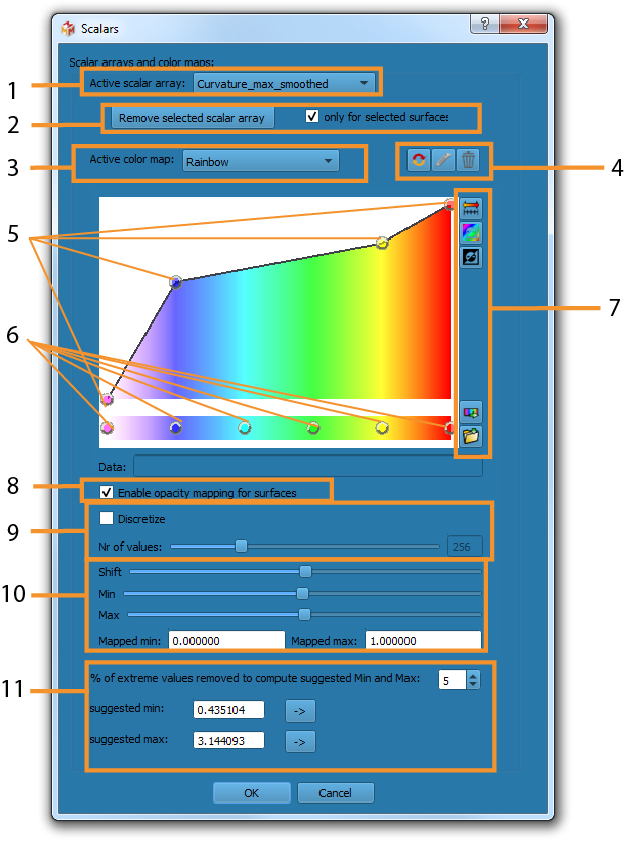
\includegraphics[scale=1]{images/11/scalar_rendering_option_window2.png}
\caption{Scalar control window. This window is divided in different subsections. \textbf{1)} chose current 3D rendered scalar array.  \textbf{2)} the active scalar array can be deleted from selected/all surface objects in this sections. \textbf{3)} chose current active color map, which transforms numbers into color and opacity on the screen. \textbf{4)} operations on the active colormap. a: reinitialize color map. b: export colors map(s) inside a .MAP file. c: change active color map name. d: delete active color map. \textbf{5)} opacity control points of the active color map. \textbf{6)} color control points of the active color map. \textbf{7)} modification controls of the active color map. a: set range to min and max. b: reverse color control points. c: reverse opacity control points. d: Save to preset = duplicate current active color map and create a new custom color map. \textbf{8)} enable/disable opacity mapping. \textbf{9)} discretize color levels, and chose number of levels. \textbf{10)} change min and max of color map. \textbf{11)} set min and max of color map based on suggested values.}	
\label{scalar_rendering_options_window}
 \end{figure}


\noindent
\textbf{\underline{Available controls:}}\\
\textbf{1: Active scalar array}: chose among the available scalars the one which will be displayed.\\\\
\noindent
\textbf{2: Remove selected scalar array}: deletes currently active scalar array from all opened surfaces, or  from selected surfaces only. This option is useful if you plan to save surfaces in the .vtk format and do not want MorphoDig to save associated scalar values (this will save some disk space).\\\\
\noindent
\textbf{3: Active color map}: chose among currently available colormaps. See Fig. \ref{change_active_color_map} for a practical example. \\\\

\begin{figure}
  \centering
  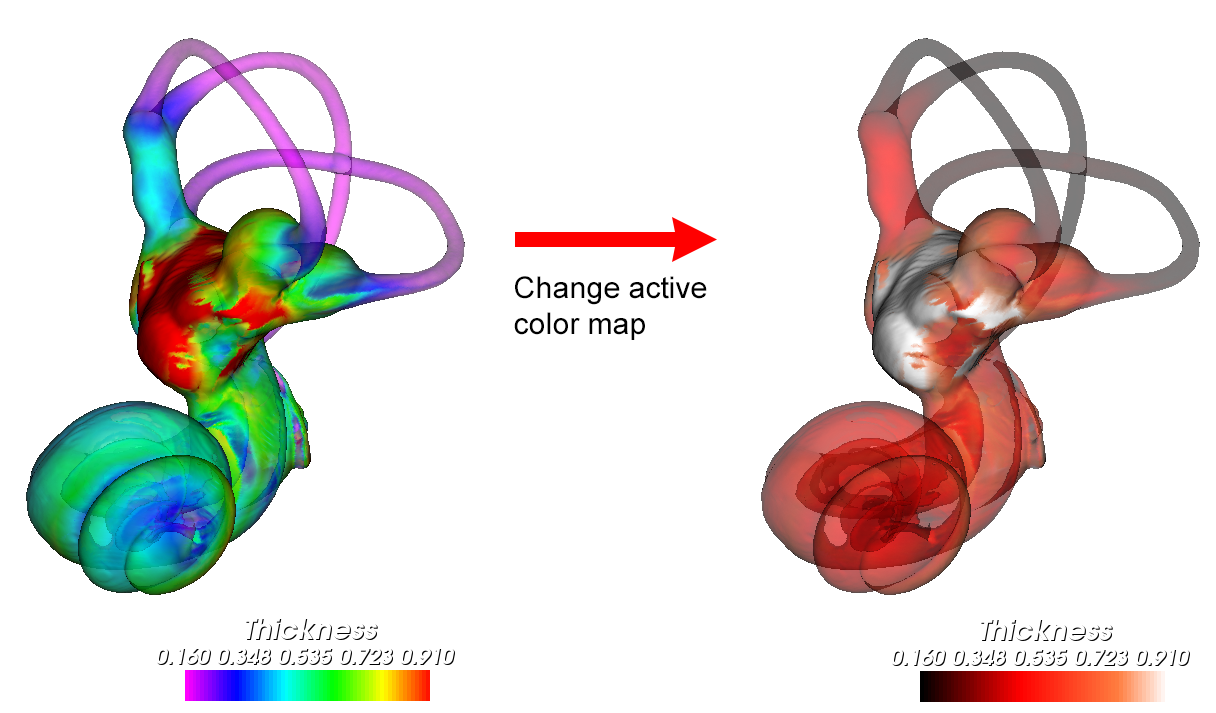
\includegraphics[scale=0.38]{images/11/change_active_color_map.png} 
	\caption{
Example of active colormap modification.  Left: left inner ear of \textit{Galago moholi}. Active scalars: thickness. Colormap: rainbow. Right: the same inner ear after the active colormap has been set to "Black-red-white".}
\label{change_active_color_map}
 \end{figure}


\noindent
\begin{minipage}{0.5\textwidth}
\textbf{4: Color map controls}: Four buttons are available. a:reinitialize color map (only possible for the 2 first predefined color maps). b: export color maps(s). When clicked, the export color map(s) dialog shows up (see Fig. \ref{export_color_maps}), in which you may define more precisely the color map(s) that should be exported.  c: change active color map name (can be only done on custom color maps). d: delete active color map (only custom color maps can be deleted).\\
\end{minipage}    
\begin{minipage}{0.5\textwidth}\centering
  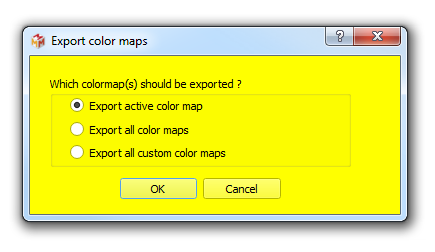
\includegraphics[scale=0.5]{images/11/export_color_maps.png}
 \captionof{figure}{Export color maps dialog.}
\label{export_color_maps}
 \end{minipage} \\\\

\noindent
\textbf{5: Opacity control points }: opacity control points of the active color map. Such control points can be added (left click on a line), deleted (select one control point using the left mouse button then press "delete") and edited (drag one control point using the left mouse button) interactively.\\\\

\noindent
\textbf{6: Color control points }: color control points of the active color map. Such control points can be added (left click on an empty zone), deleted (select one control point using the left mouse button then press "delete") and edited (drag one control point using the left mouse button) interactively.\\\\
\noindent
\textbf{7: additional color map controls}. From top to bottom. a: set colormap range to match the global active scalar min and max found for all currently opened surfaces. b: reverse color color control points (see Fig. \ref{invert_colors}). c: reverse opacity control points (see Fig. \ref{invert_opacities}). d:  Save to preset = duplicate current active color map and create a new custom color map.duplicate current active color map and create a new custom color map. \\\\



\begin{figure}
  \centering
  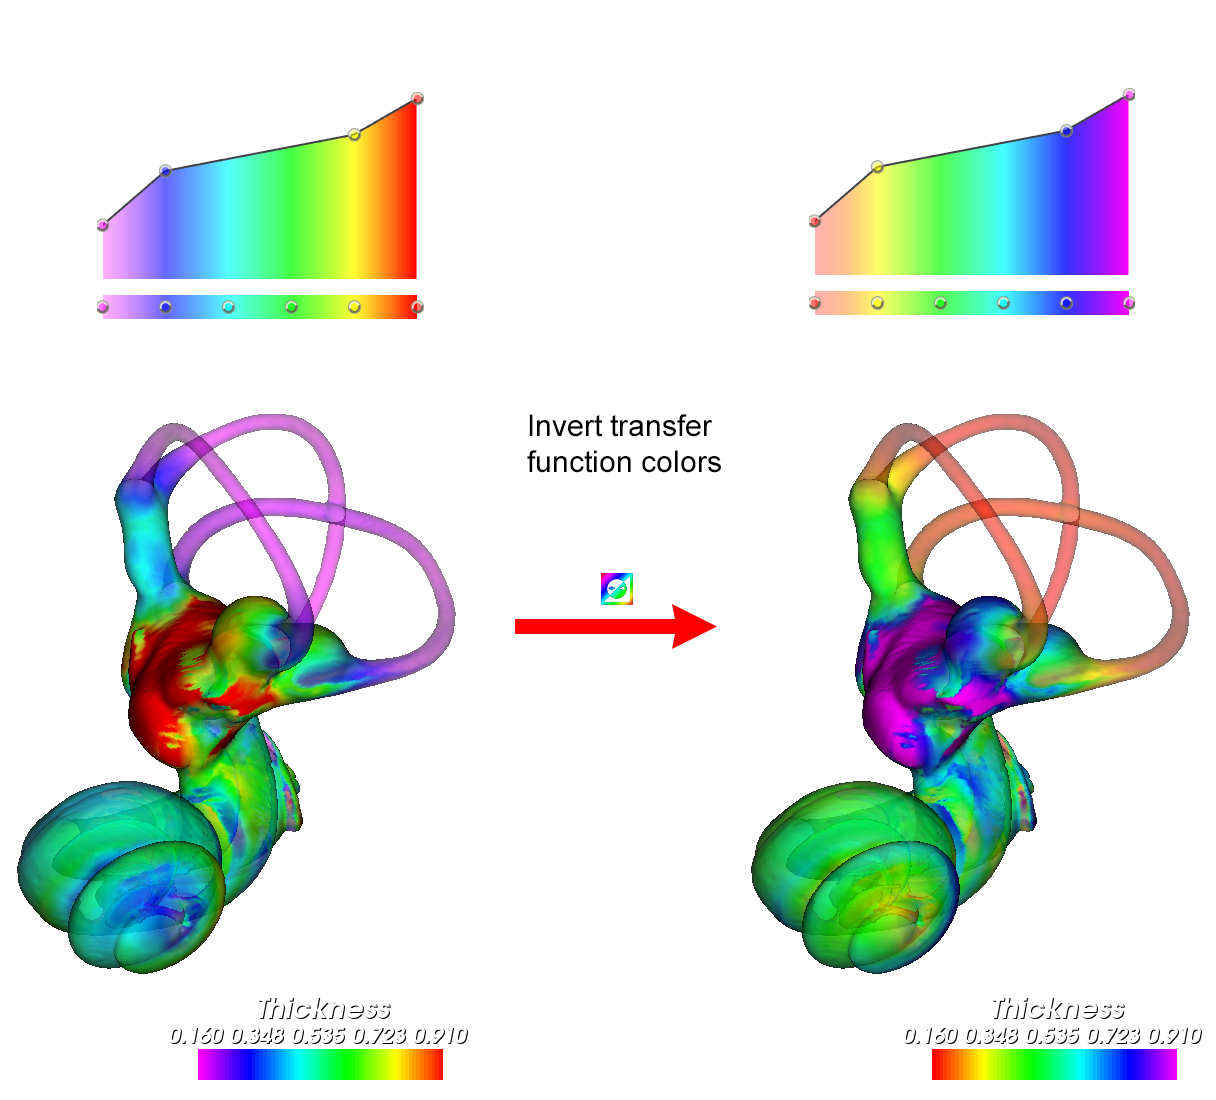
\includegraphics[scale=0.38]{images/11/invert_colors.png} 
	\caption{
Example of color inversion of a colormap.  Left: left inner ear of \textit{Galago moholi}. Active scalars: thickness. Colormap: rainbow. Right: the same inner ear after the color control points of the rainbow colormap have been reversed.}
\label{invert_colors}
 
\end{figure}

\begin{figure}
  \centering
  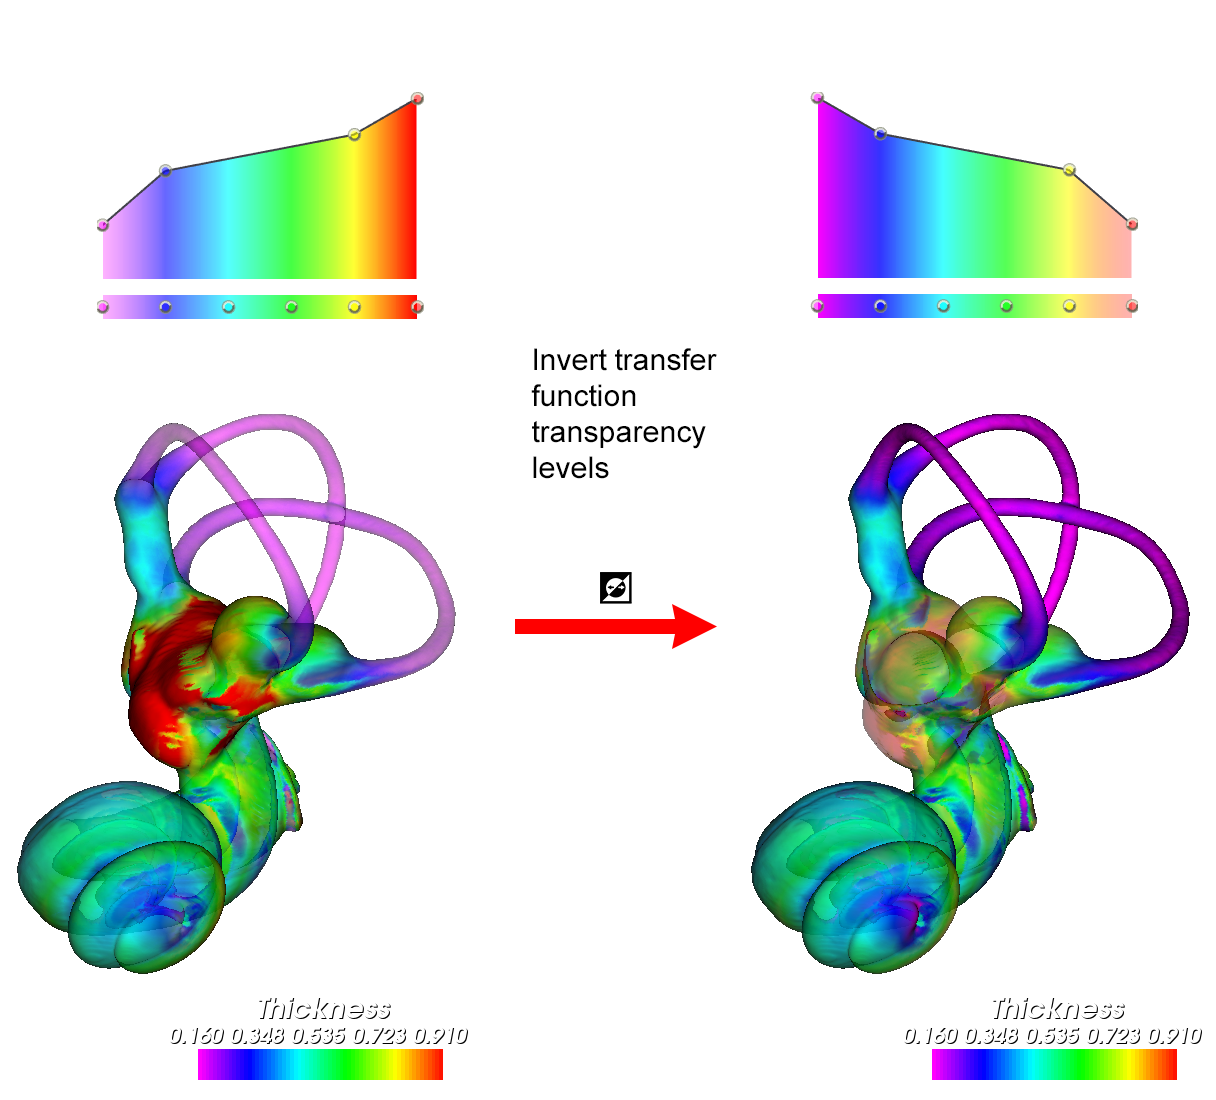
\includegraphics[scale=0.38]{images/11/invert_transparency.png} 
	\caption{
	Example of opcacity inversion of a colormap.  Left: left inner ear of \textit{Galago moholi}. Active scalars: thickness. Colormap: rainbow. Right: the same inner ear after the opacity leveles of the rainbow colormap have been reversed.}
\label{invert_opacities}
 
\end{figure}

\noindent
\textbf{8: enable/disable opacity mapping.} When opacity mapping is disabled, all surface objects are rendered using their "global" transparency level.\\\\

\noindent
\textbf{9: discretize color levels}, and chose number of levels. See Fig. \ref{discretize_example} for a practical example.\\\\
\begin{figure}
  \centering
  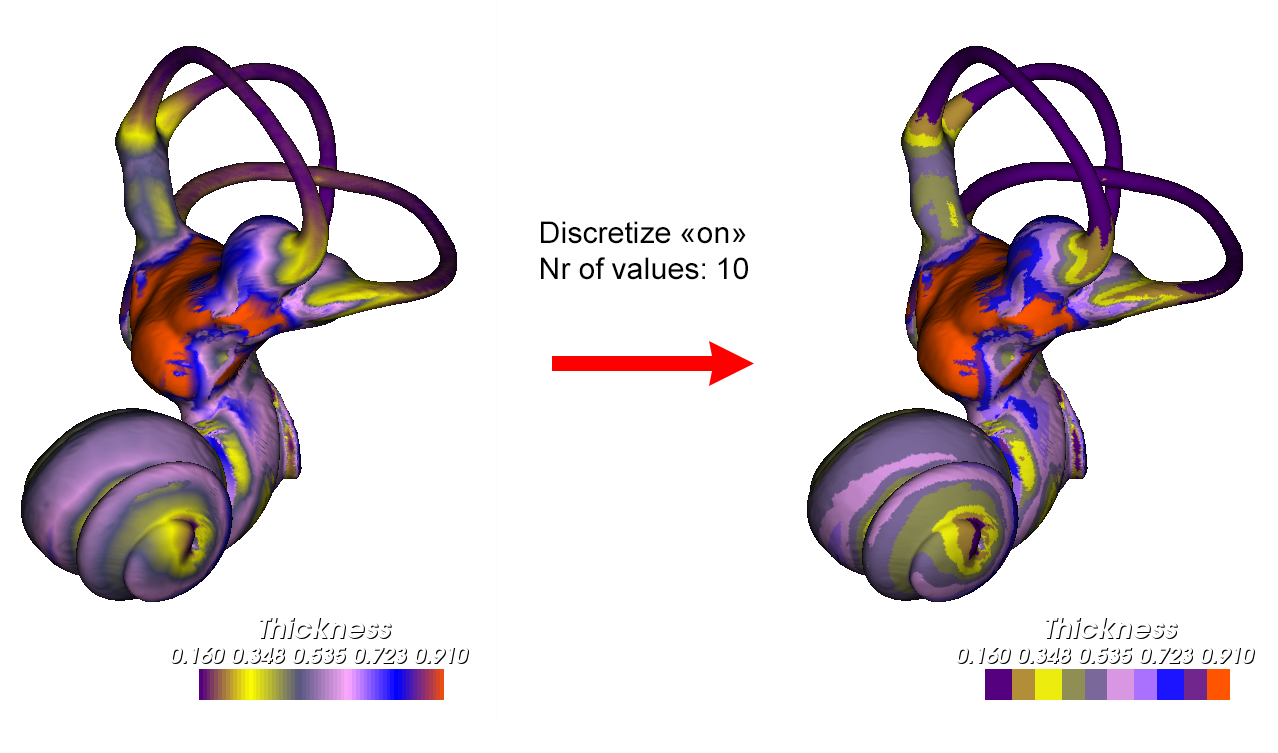
\includegraphics[scale=0.38]{images/11/discretize_on.png} 
	\caption{
Example of colormap discretization.  Left: left inner ear of \textit{Galago moholi}. Active scalars: thickness. Colormap: custom. Right: the same inner ear after the "discretize" option has been turned on, and the nr of values set to 10.}
\label{discretize_example}
 
\end{figure}

\noindent
\textbf{10: change min and max of color map.} You may use these sliders to change the minimal and maximal values of the active color map. By default, all colormaps range between 0 (min) and 1 (max), which may not be the most appropriate range to display a given scalar array. \\\\ 


\noindent
\textbf{11: set min and max of color map based on suggested values.} As stated above, by default, all colormaps range between 0 (min) and 1 (max), which may not be the most appropriate range to display a given scalar array. You may set the minimal and maximal values of the active colormap based on suggested values, which are computed automatically based on the currently opened surface objects, and which are computed in order to use the color scale at its best. See Fig. \ref{accept_suggested_min_max} for a practical example. \\\\

\begin{figure}
  \centering
  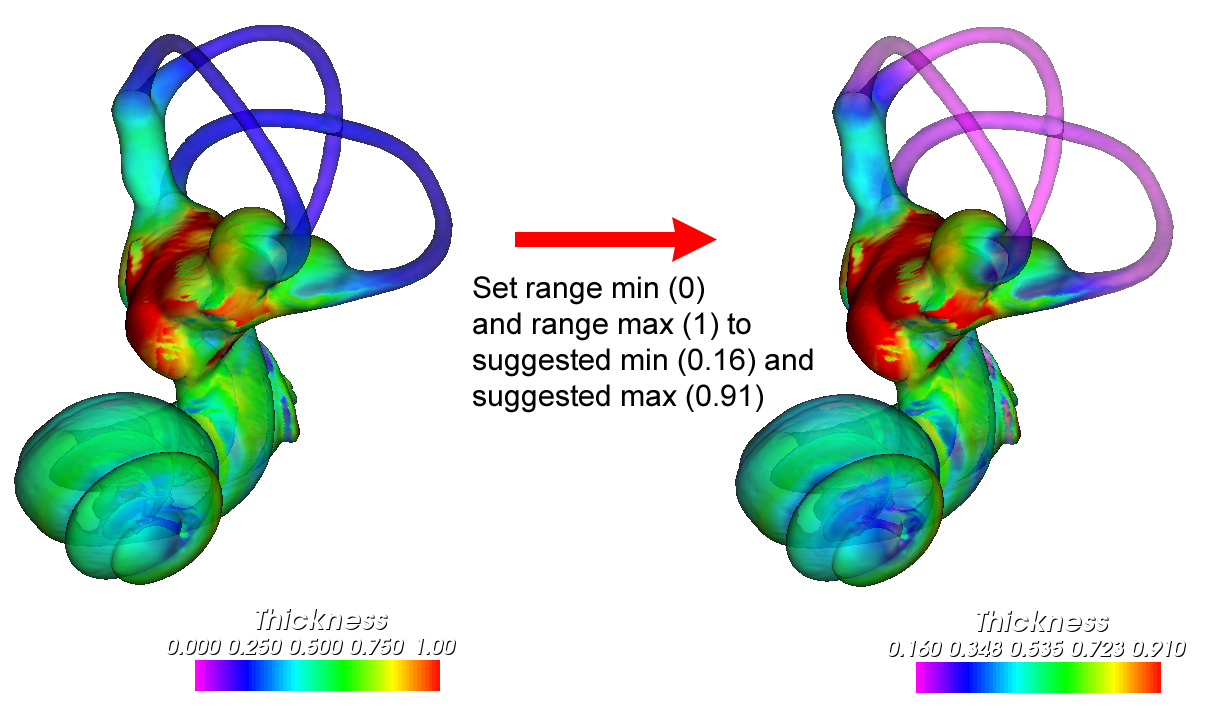
\includegraphics[scale=0.38]{images/11/accept_suggested_min_max.png} 
	\caption{
Example of suggested min and max usage. Left: Left inner ear of \textit{Galago moholi}. Active scalars: thickness. Colormap: rainbow. Te rainbow colormap is set as by default to range between 0 (min) and 1 (max). Right: the same inner ear after the rainbow colormap range has been modified based on suggested min (0.16) and suggested max (0.91) values.}
\label{accept_suggested_min_max}
 
\end{figure}
\noindent




\section{Compute distance from camera for each selected surface}
\noindent
Computes distance (=depth) from camera for all vertices of all selected surfaces. This option may offer a better
perception of the 3D structure of an object on a 2D screen representation. This option also makes it possible to compute an elevation map. See Fig. \ref{camera_distance} for a practical example. 
 
\begin{figure}
  \centering
  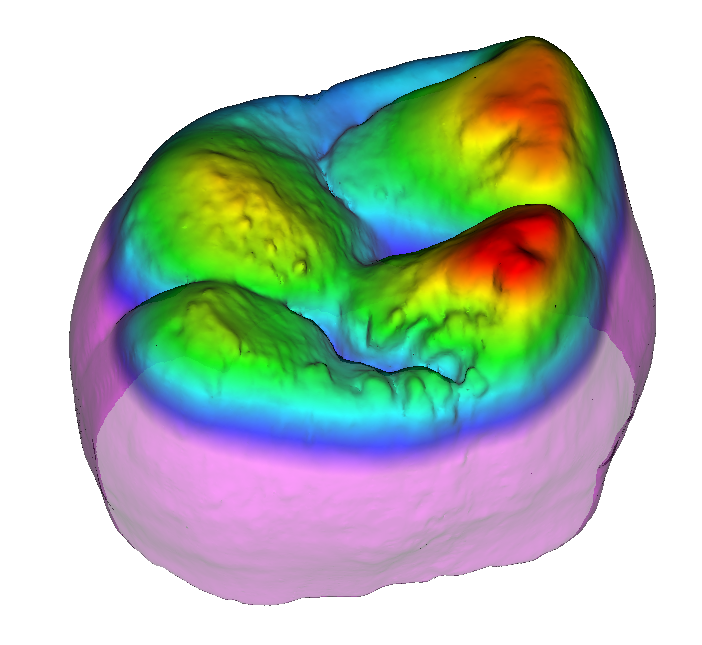
\includegraphics[scale=0.38]{images/11/camera_distance_example.png} 
	\caption{
Example of camera distance scalar array. Displayed specimen: upper outer enamel surface of a second upper molar of \textit{Homo sapiens}.}
\label{camera_distance}
 
\end{figure}
\noindent


\noindent



\section{Compute thickness within each selected surface}
\begin{minipage}{0.5\textwidth}
Thickness within an object (see Fig. \ref{thickness_within_dialog}) is defined the following way: for a
given vertex, the minimal distance between this vertex and other
vertices in the direction opposite to that of the surface's normal. In order to minimize computation time, a maximal
distance (Maximal thickness (size unit) ) is asked to the user, in order
to reduce the amount of vertices investigated at a given location. Also, in order to avoid to take into account only relevant vertices in that computation, an angular limit between investigated vertex normals (by default: 70\degree) is asked. Finally, a smoother scalar array output can be produced by setting the "thickness" value as the average of the distance found between a number of closest vertices found. See Fig. \ref{thickness_examples}-A for a practical example. 
 
\end{minipage}    
\begin{minipage}{0.5\textwidth}\centering
 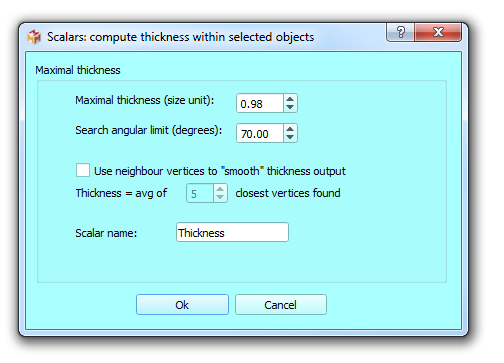
\includegraphics[scale=0.5]{images/11/thickness_within_dialog.png}
 \captionof{figure}{Thickness within a given surface.}
\label{thickness_within_dialog}
 \end{minipage} 


\begin{figure}
  \centering
  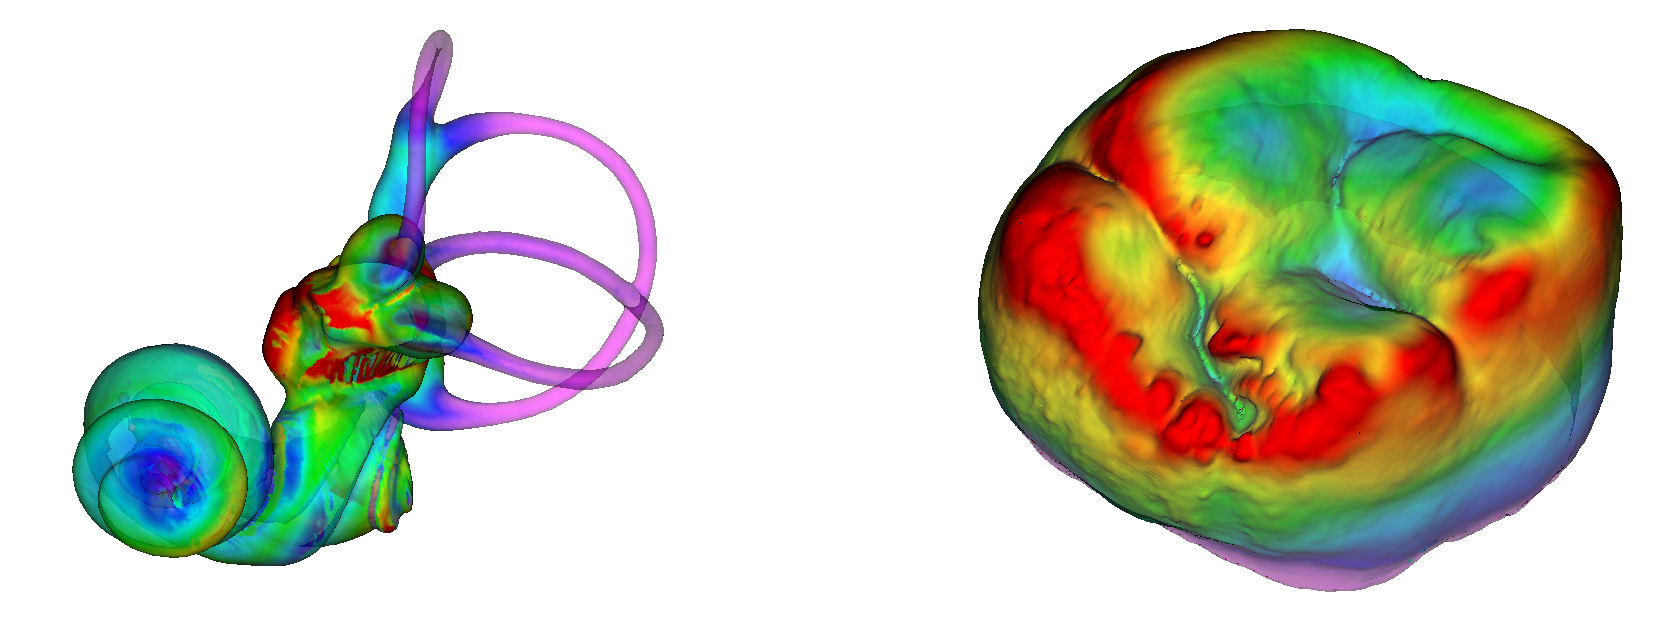
\includegraphics[scale=0.28]{images/11/thickness_examples.png} 
	\caption{
Examples of thickness computation. A: thickness within object. Specimen: left inner ear of \textit{Galago moholi}. B: thickness between the outer enamel surface (OEJ) and the enamel-dentine junction (EDJ) of a second upper molar of \textit{Homo sapiens}.}
\label{thickness_examples}
 
\end{figure}




\section{Compute thickness between two surfaces}

\noindent
\begin{minipage}{0.5\textwidth}
Thickness between two objects is defined the following way (see Fig. \ref{thickness_between_dialog}):
for a given vertex of the impacted object, the minimal distance
between this vertex and other vertices of the observed surface in
the same direction (if "invert normals of observed object" option is unchecked) or in the opposite direction (if "invert normals of observed object" option is checked) to that of the impacted surface's normal is computed. Again, in order to minimize computation time, a maximal distance (Maximal thickness (size unit) ) is asked to the user, in order to reduce the amount of vertices investigated at a given location. Also, in order to avoid to take into account only relevant vertices in that computation, an angular limit between investigated vertex normals (by default: 70\degree) is asked. Finally, a smoother scalar array output can be produced by setting the "thickness" value as the average of the distance found between a number of closest vertices found. See Fig. \ref{thickness_examples}-B for a practical example.
\end{minipage}    
\begin{minipage}{0.5\textwidth}\centering
  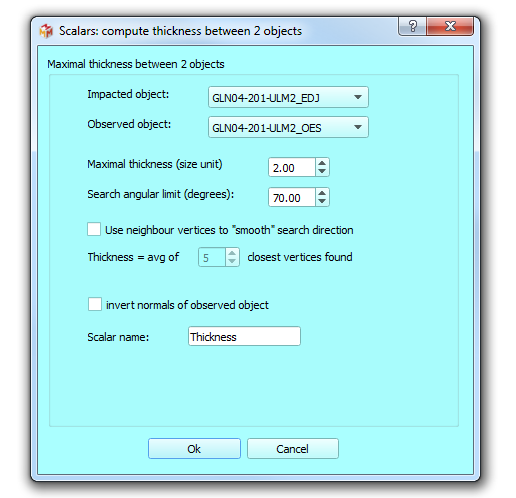
\includegraphics[scale=0.5]{images/11/thickness_between_dialog.png}
 \captionof{figure}{Thickness between 2 surfaces window}
\label{thickness_between_dialog}
 \end{minipage} 
\noindent


\section{Compute distance between two surfaces}
\noindent
\begin{minipage}{0.5\textwidth}
Vertex closest distance between two objects is computed as the minimal distance between all vertices  vertex and other vertices of the observed surface, regardless of the direction. This option may be relevant if you want to compare the same object twice (for instance the object before and after some alteration) or want to compare two objects of very similar shape (for instance two inner ears belonging to two specimens of the same species). Before computing a distance map, it is strongly advised, in a preliminary step, to align the two compared surfaces (see section \ref{surface_alignment_section} p.\pageref{surface_alignment_section}). The computed distance can be somewhat "smoothed" by being defined as the average value of a given number of closest vertices. Again, in order to minimize computation time, a maximal distance (in size unit) is asked to the user, in order to reduce the amount of vertices investigated at a given location. See Fig. \ref{distance_between_example} for a practical example.
\end{minipage}    
\begin{minipage}{0.5\textwidth}\centering
  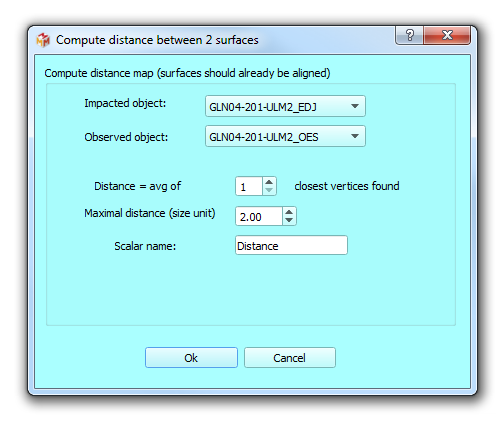
\includegraphics[scale=0.5]{images/11/distance_between_dialog.png}
 \captionof{figure}{Distance between 2 surfaces window}
\label{distance_between_dialog}
 \end{minipage} 
\noindent


\begin{figure}
  \centering
  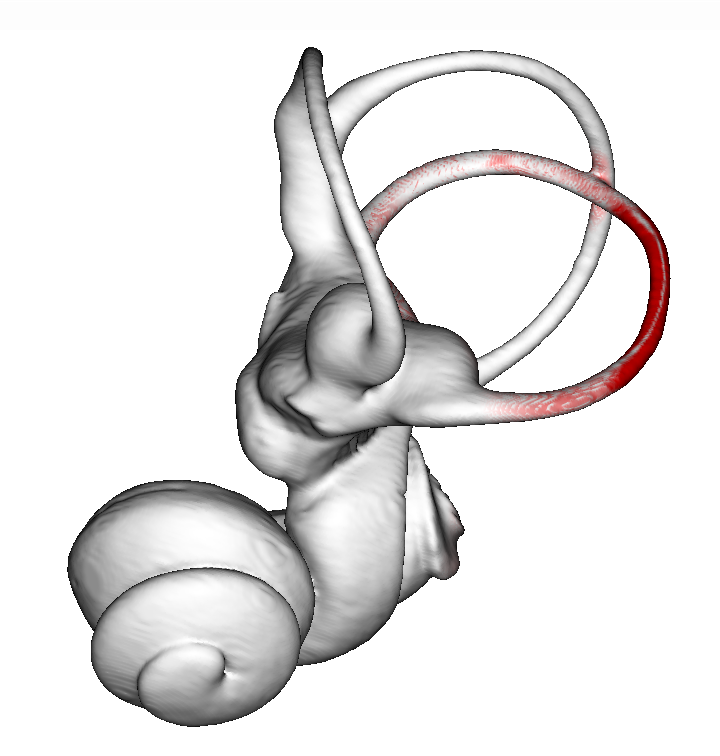
\includegraphics[scale=0.28]{images/11/distance_between_example.png} 
	\caption{
Example of distance map between two surfaces. An inner ear of \textit{Galago moholi} was virtually distorted in the lateral canal region. The corresponding representation of the deformation is shown here using a distance map: in red can we identify the most distorted regions.}
\label{distance_between_example}
 
\end{figure}



\section{Compute curvature for each selected surface}
\noindent
\begin{minipage}{0.5\textwidth}
vtkCurvatures filter is implied in this option.\\
vtkCurvatures filter offers 4 ways to compute surface's
curvature at each vertex (see Fig. \ref{curvatures}):\\
- Principal maximal curvature\\
- Principal minimal curvature\\
- Gaussian curvature\\
- Mean curvature.\\
See vtkCurvatures' documentation for further details.

\end{minipage}    
\begin{minipage}{0.5\textwidth}\centering
  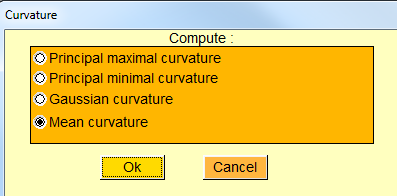
\includegraphics[scale=0.5]{images/Scalars_renreding/Curvature_window.png}
 \captionof{figure}{Curvature window}
\label{curvature_window}
 \end{minipage} 
\noindent

\begin{figure}
  \centering
  \includegraphics[scale=0.3]{images/Scalars_renreding/Curvatures.pdf} 
	\caption{
Examples of 3D rendering of ``Curvature" scalars. Scalar mode is active, the rainbow color scale is used. Specimen : enamel dentine junction (EDJ) of the second superior molar of a juvenile medieval human from Sains-en-Gohelle (France). Specimen number : SP07. Image credit: Mona Le Luyer (PACEA, Bordeaux).}
\label{curvatures}
 
\end{figure}

\section{Compute complexity for each selected surface}


\section{Smooth active scalars for each selected surface}
Active scalars are ``smoothed" the following way : for each vertex, a new scalar value is computed as
the mean of the scalar values of all neighbouring vertices (see Fig. \ref{smoothing_scalars}).
\begin{figure}
  \centering
  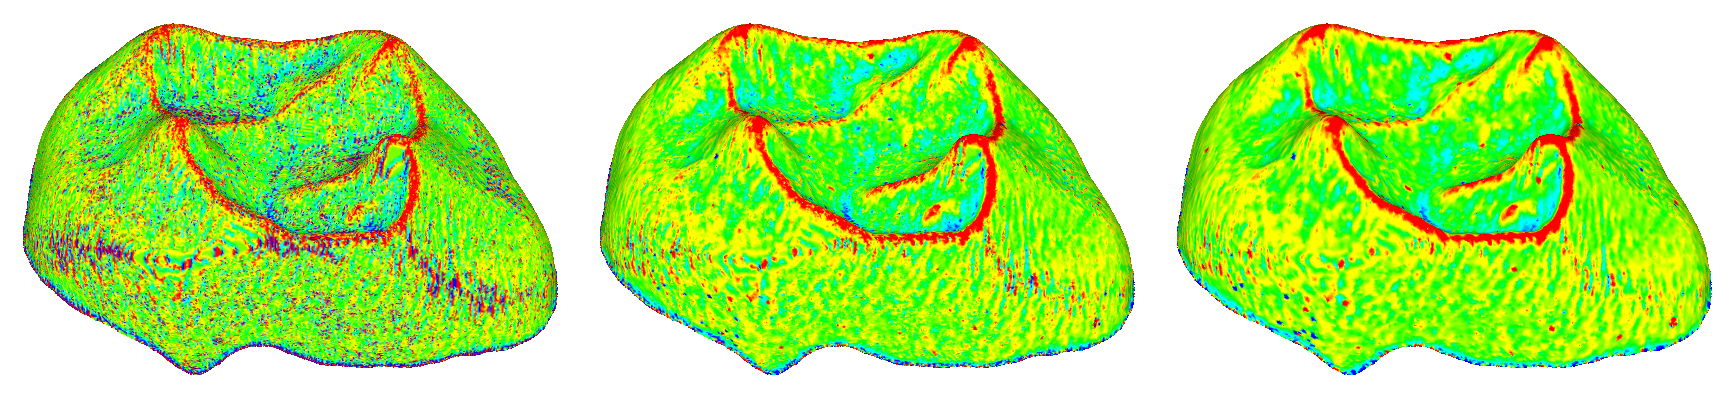
\includegraphics[scale=0.25]{images/Scalars_renreding/Smooth_012.png} 
	\caption{Smoothing scalars. Examples of 3D rendering of ``Mean Curvature" scalars. Scalar mode is active, the rainbow color scale is used. Left : ``raw" mean curvature. Middle : mean curvature scalars smoothed once. Right : mean curvature scalars smoothed twice. Specimen: EDJ of SP07 specimen.}
\label{smoothing_scalars}
 
\end{figure}




\section{Show scalar rendering options window.}





















\section{Saving and loading scalars.}
Computed scalars can be saved inside the .vtk surface files. In order to access scalar values into other software (such as a text editor), save the .vtk files in ASCII format. Saved scalars can be reloaded into ISE-MeshTools. Saving surfaces into .vtk format provides an efficient means to store and exchange
computed scalars.
